\documentclass[10pt]{article}
\usepackage[english]{babel}
\usepackage{../../../meta-inf/lib/naproche}
\usepackage{amssymb}
\usepackage{mathtools} % for \coloneq

\usepackage{stex-highlighting}
\providebool{emph} % "\newbool{emph}" does not work...
\setbool{emph}{false}
\colorlet{emphcolor}{violet}
\let\oldemph\emph
\renewcommand\emph[1]{\setbool{emph}{true}\ifbool{forthel}{\textcolor{emphcolor}{\itshape#1}}{\oldemph{#1}}\setbool{emph}{false}}
\renewcommand{\varemph}[1]{\ifbool{emph}{\textcolor{emphcolor}{#1}}{\textcolor{black}{#1}}}

\usepackage[right=6cm,left=3cm,bottom=3cm,marginparwidth=5cm]{geometry}

\usepackage{fancyhdr}
\renewcommand{\sectionmark}[1]{\markboth{#1}{}} 
\def\libarchive{}
\pagestyle{fancy}
\fancyhead[L]{\libarchive}
\fancyhead[C]{\nouppercase\leftmark}  % section title
\fancyhead[R]{\thepage}               % page number
\fancyfoot[C]{}                       % No page number in footer

\usepackage[nobottomtitles]{titlesec}
\titlespacing*{\section}{0pt}{30pt}{0pt}
\titlespacing*{\subsection}{0pt}{30pt}{0pt}
\titlespacing*{\subsubsection}{0pt}{30pt}{0pt}

\documentclass[12pt,oneside]{book}

\usepackage[foundations]{../../lib/tex/naproche}
\usepackage{../../lib/tex/libraries}
\usepackage{graphicx}
\usepackage{float}
\usepackage{caption}
\usepackage{footnote}

\makesavenoteenv{tabular} % Make footnotes work in tabular environments


\title{Foundations of Mathematics}
\author{Marcel Schütz}
\date{2022}

\begin{document}
  \maketitle

  \tableofcontents

  \begin{figure}[H]
    \centering
    \fbox{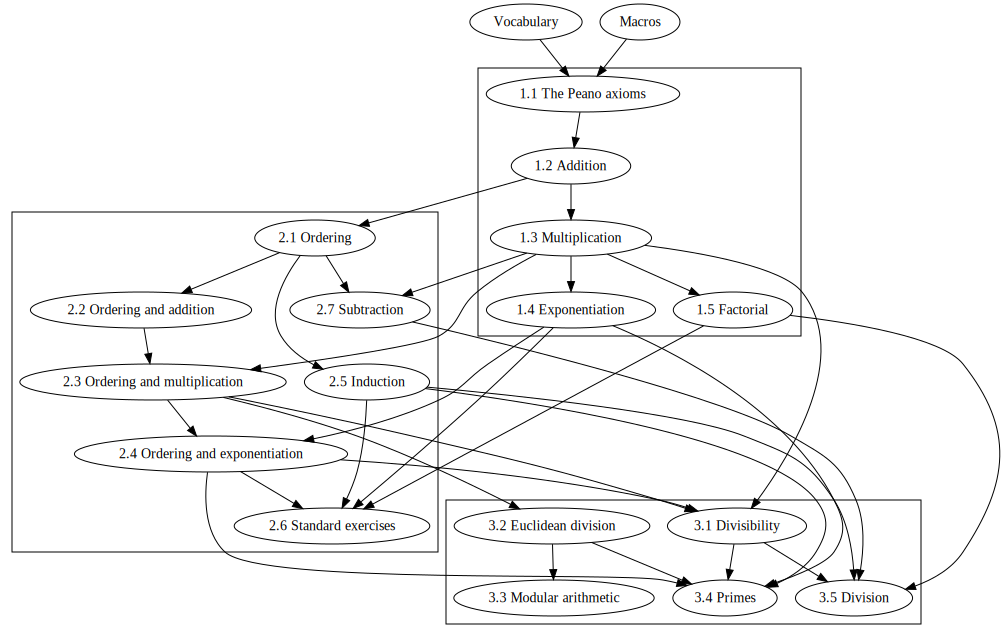
\includegraphics[width=0.9\linewidth]{./dependency-graph/graph.png}}
    \caption*{Interdependencies of the chapters}
  \end{figure}


  \section*{Introduction}

  This is a library providing a foundation of mathematics based on a
  Kelley-Morse like class theory with urelements.
  It introduces common operations on classes like unions or intersections
  (\cref{chapter:classes}) together with detailed proofs of their algebraic
  properties (\cref{chapter:computation-laws-for-classes}), the symmetric
  difference of two classes (\cref{chapter:symmetric-difference}) and the
  notions of ordered pairs and Cartesian products
  (\cref{chapter:pairs-and-products}) as well as proofs of the algebraic
  properties of the latter (\cref{chapter:computation-laws-for-products}).
  Moreover, it provides common operations on maps (\cref{chapter:maps}), various
  properties of images and preimages (\cref{chapter:image-and-preimage}) and the
  notions of injectivity, surjectivity, bijectivity
  (\cref{chapter:injections-surjections-bijections}) and invertibility of maps
  (\cref{chapter:invertible-maps}).
  The library provides an axiom system characterizing sets (\cref{chapter:sets})
  and, furthermore, it covers the notions of binary relations
  (\cref{chapter:binary-relations}), fixed-points of subset preserving maps
  (\cref{chapter:fixed-points}), including and equinumerosity
  (\cref{chapter:equinumerosity}).

  As two famous results it includes the Knaster-Tarski fixed point theorem
  (\cref{FOUNDATIONS_12_8420450166112256}) and the Cantor-Schröder-Bernstein
  theorem (\cref{FOUNDATIONS_13_1913663275401216}).

  \paragraph*{Usage.}
  At the very beginning of each chapter you can find the name of its source
  file, e.g. \path{foundations/sections/01_classes.ftl.tex} for
  \cref{chapter:classes}. This filename can be used to import the chapter via
  \Naproche's \texttt{readtex} instruction to another ForTheL text, e.g.:
  \begin{center}
    \verb`[readtex \path{foundations/sections/01_classes.ftl.tex}]`
  \end{center}

  \paragraph*{Checking times.}
  The checking times for each of the chapters may vary from computer to
  computer, but on mid-range hardware they are likely to be similar to those
  given in table below:

  \begin{center}
    \begin{tabular}{c|c|c}

      & \multicolumn{2}{c}{\textbf{Checking time}}
      \\
      \textbf{Chapter}
      & \textbf{without dependencies}     & \textbf{with dependencies}
      \\ \hline
      \ref{chapter:classes}
      & 00:04 min                         & 00:04 min
      \\
      \ref{chapter:computation-laws-for-classes}
      & 00:12 min                         & 00:16 min
      \\
      \ref{chapter:symmetric-difference}
      & 00:32 min                         & 00:48 min
      \\
      \ref{chapter:pairs-and-products}
      & 00:08 min                         & 00:12 min
      \\
      \ref{chapter:computation-laws-for-products}
      & 01:36 min                         & 01:56 min
      \\
      \ref{chapter:maps}
      & 01:13 min                         & 01:25 min
      \\
      \ref{chapter:image-and-preimage}
      & 01:28 min                         & 02:53 min
      \\
      \ref{chapter:injections-surjections-bijections}
      & 00:38 min                         & 02:03 min
      \\
      \ref{chapter:invertible-maps}
      & 02:20 min                         & 04:23 min
      \\
      \ref{chapter:sets}
      & 02:17 min                         & 06:40 min
      \\
      \ref{chapter:binary-relations}
      & 00:14 min                         & 06:54 min
      \\
      \ref{chapter:fixed-points}
      & 00:33 min                         & 07:13 min
      \\
      \ref{chapter:equinumerosity}
      & 01:48 min                         & 09:01 min
    \end{tabular}
  \end{center}


  \subfile{sections/01_classes.ftl.tex}
  \subfile{sections/02_computation-laws-for-classes.ftl.tex}
  \subfile{sections/03_symmetric-difference.ftl.tex}
  \subfile{sections/04_pairs-and-products.ftl.tex}
  \subfile{sections/05_computation-laws-for-products.ftl.tex}
  \subfile{sections/06_maps.ftl.tex}
  \subfile{sections/07_image-and-preimage.ftl.tex}
  \subfile{sections/08_injections-surjections-bijections.ftl.tex}
  \subfile{sections/09_invertible-maps.ftl.tex}
  \subfile{sections/10_sets.ftl.tex}
  \subfile{sections/11_binary-relations.ftl.tex}
  \subfile{sections/12_fixed-points.ftl.tex}
  \subfile{sections/13_equinumerosity.ftl.tex}
\end{document}

\usepackage{amssymb}

\newcommand{\Nat}{\mathbb{N}}
\newcommand{\Prime}{\mathbb{P}}
\renewcommand{\succ}{\textrm{succ}}
\newcommand{\pred}{\textrm{pred}}
\newcommand{\add}{\textrm{add}}
\newcommand{\mul}{\textrm{mul}}
\renewcommand{\exp}{\textrm{exp}}
\newcommand{\fac}{\textrm{fac}}
\renewcommand{\div}{\mathop{\textrm{div}}}
\renewcommand{\mod}{\mathop{\textrm{mod}}}

\begin{document}
  \begin{imports}
    \begin{forthel}
      %[prove off][check off]
      [read \path{libraries/source/foundations/systems-of-sets.ftl.tex}]
      [read \path{libraries/source/foundations/finite-and-infinite-classes.ftl.tex}]
      %[prove on][check on]
    \end{forthel}
  \end{imports}


  \section*{Closure Under Finite Unions}

  \begin{forthel}
    \begin{definition}[id=FOUNDATIONS_14_7040118193913856,printid]
      Let $X$ be a system of sets.
      $X$ is closed under finite unions iff $\bigcup U \in X$ for every nonempty finite subclass $U$ of $X$.
    \end{definition}
  \end{forthel}

  \begin{forthel}
    \begin{proposition}[id=FOUNDATIONS_17_4164024962908160,printid]
      Let $X$ be a system of sets.
      $X$ is closed under finite unions iff $U \cup V \in X$ for every $U, V \in X$.
    \end{proposition}
    \begin{proof}
      Case $X$ is closed under finite unions.
        Let $U, V \in X$.
        Then $\set{U, V}$ is a nonempty finite subclass of $X$.
        Hence $U \cup V = \bigcup \set{U, V} \in X$.
      End.
  
      Case $U \cup V \in X$ for every $U, V \in X$.
        Define $\Phi = \{ n \in \Nat \mid \bigcup U \in X$ for every nonempty subclass $U$ of $X$ that has $n$ elements $\}$.
  
        (1) $\Phi$ contains $0$.
  
        (2) For every $n \in \Phi$ we have $n + 1 \in \Phi$. \\
        Proof.
          Let $n \in \Phi$.
          Then $\bigcup U \in X$ for every nonempty subclass $U$ of $X$ that has $n$ elements.
  
          Let us show that $\bigcup U \in X$ for every nonempty subclass $U$ of $X$ that has $n + 1$ elements.
  
            Case $n = 0$. Obvious.
  
            Case $n \neq 0$.
              Let $U$ be a nonempty subclass of $X$ such that $U$ has $n + 1$ elements.
              Take a bijection $f$ between $\{1, \dots, n + 1 \}$ and $U$.
              We have $\{ 1, \dots, n + 1 \} = \{ 1, \dots, n \} \cup \set{n + 1}$.
              Take $V = f[\{ 1, \dots, n \}]$.
              We have $\{ 1, \dots, n \} \subseteq \{ 1, \dots, n + 1 \}$.
  
              Let us show that $V \subseteq U$.
                Let $x \in V$.
                Take $k \in \{ 1, \dots, n \}$ such that $x = f(k)$.
                Indeed we can show that there exists a $k \in \{ 1, \dots, n \}$ such that $x = f(k)$.
                  Assume the contrary.
                  Then $x \neq f(k)$ for all $k \in \{ 1, \dots, n \}$.
                  Hence $x \notin f[\{ 1, \dots, n \}] = V$.
                  Contradiction.
                End.
                Hence $x \in U$.
                Indeed $x \in f[\{ 1, \dots, n + 1 \}]$.
              End.

              $V$ is nonempty.
              Indeed $f(1) \in f[\{ 1, \dots, n \}]$.
              Indeed $1 \in \{ 1, \dots, n \}$.
              Hence $f \restriction \{ 1, \dots, n \}$ is a bijection between $\{ 1, \dots, n \}$ and $V$ (by \cref{FOUNDATIONS_08_647446231252992}).
              Thus $V$ has $n$ elements.
              Consequently $\bigcup V \in X$.

              Let us show that $U = V \cup \set{f(n + 1)}$. \\
                (1) $f[A \cup B] = f[A] \cup f[B]$ for all $A, B \subseteq \dom(f)$.

                (2) $f[\set{a}] = \set{f(a)}$ for all $a \in \dom(f)$.

                Hence $U
                  = f[\dom(f)]
                  = f[\{ 1, \dots, n + 1 \}]
                  = f[\{ 1, \dots, n \} \cup \set{n + 1}]
                  = f[\{ 1, \dots, n \}] \cup f[\set{n + 1}]
                  = f[\{ 1, \dots, n \}] \cup \set{f(n + 1)}
                  = V \cup \set{f(n + 1)}$.
                Indeed $n + 1 \in \dom(f)$ and $\{ 1, \dots, n \}, \set{1 + n} \subseteq \dom(f)$.
              End.
  
              Let us show that $\bigcup (A \cup B) = (\bigcup A) \cup (\bigcup B)$ for any nonempty systems of sets $A, B$.
                Let $A, B$ be nonempty systems of sets.
                $\bigcup (A \cup B) \subseteq (\bigcup A) \cup (\bigcup B)$.
                $((\bigcup A) \cup (\bigcup B)) \subseteq \bigcup (A \cup B)$. %!
              End.
  
              Let us show that $f(n + 1)$ and $f(k)$ are sets for every $k \in \{ 1, \dots, n \}$.
                Let $k \in \{ 1, \dots, n \}$.
                Then $f(k), f(n + 1) \in U$.
                Hence $f(k)$ and $f(n + 1)$ are sets.
              End.

              Hence $V$ and $\set{f(n + 1)}$ are nonempty systems of sets.
              Thus $\bigcup U
                = \bigcup (V \cup \set{f(n + 1)})
                = (\bigcup V) \cup (\bigcup \set{f(n + 1)})
                = (\bigcup V) \cup f(n + 1)
                \in X$.
            End.
          End.
        Qed.

        Therefore $\Phi$ contains every natural number (by \printref{ARITHMETIC_01_4764664342773760}).
        Thus $\bigcup U \in X$ for every nonempty finite subclass $U$ of $X$.
        Consequently $X$ is closed under finite unions.
      End.
    \end{proof}
  \end{forthel}
\end{document}
